%==============================================================================
% LaTeXの処理に関するおまじない (マジックコメント)
%==============================================================================
% !TEX encoding = UTF-8
% !TEX ts-program = platex

%==============================================================================
% ドキュメントクラス
%==============================================================================
\documentclass[11pt, dvipdfmx]{jsarticle}

%==============================================================================
%【必須級】便利なパッケージたち
%==============================================================================

%----- ページ設定 -----
\usepackage[
    top=20mm,
    bottom=20mm,
    left=20mm,
    right=20mm
]{geometry}

%----- フォント設定 -----
\usepackage[T1]{fontenc} %【警告対策①】欧文フォントエンコーディングを指定
\usepackage{newtxtext}
\usepackage{courier} 
\usepackage{newtxmath}
\usepackage{textcomp}
% \usepackage{newtxtt}

%----- 数式関連 -----
\usepackage{amsmath}
\usepackage{siunitx}
\usepackage[detect-all]{siunitx} % フォントを自動検出させて警告を消す!

%----- 図表・画像関連 -----
% [demo]オプションで画像ファイルが無くてもコンパイルOKにしてるよ
\usepackage{graphicx} 
\usepackage{tikz}
\usepackage{pgfplots}
\pgfplotsset{compat=1.18}
\usepackage{here}
\usepackage{booktabs}
\usepackage{float}

%----- ソースコード表示 -----
\usepackage{listings}
\lstset{
    basicstyle=\ttfamily\small,
    breaklines=true,
    frame=single,
    commentstyle={\itshape \color[gray]{0.5}},
    keywordstyle={\bfseries \color{blue}},
    stringstyle={\color{red}},
    showstringspaces=false,
    numbers=left,
    numberstyle=\tiny\color[gray]{0.5},
    captionpos=b
}
% \usepackage{lmodern}

%----- その他便利機能 -----
\usepackage[dvipdfmx, unicode]{hyperref}
\usepackage{pxjahyper} % ブックマークの日本語文字化け対策
\usepackage{cleveref}
\crefname{figure}{図}{図}
\crefname{table}{表}{表}
\crefname{section}{第}{第}
\crefname{equation}{式}{式}

%==============================================================================
% ドキュメント情報
%==============================================================================
\title{ここにレポートのタイトルを記入}
\author{地球総合工学科 \quad B3 \quad 08C23031 \quad 古賀 光一朗}
\date{\today}

%==============================================================================
% 本文開始
%==============================================================================
\begin{document}

\maketitle

\section{短辺方向のGMの計算}
10/14, "寸法を一旦決め打ちしないといろいろな値が決まらない"ということで、一旦未知数を文字でおいてGMを計算してみた。

\begin{figure}[H]
    \centering
    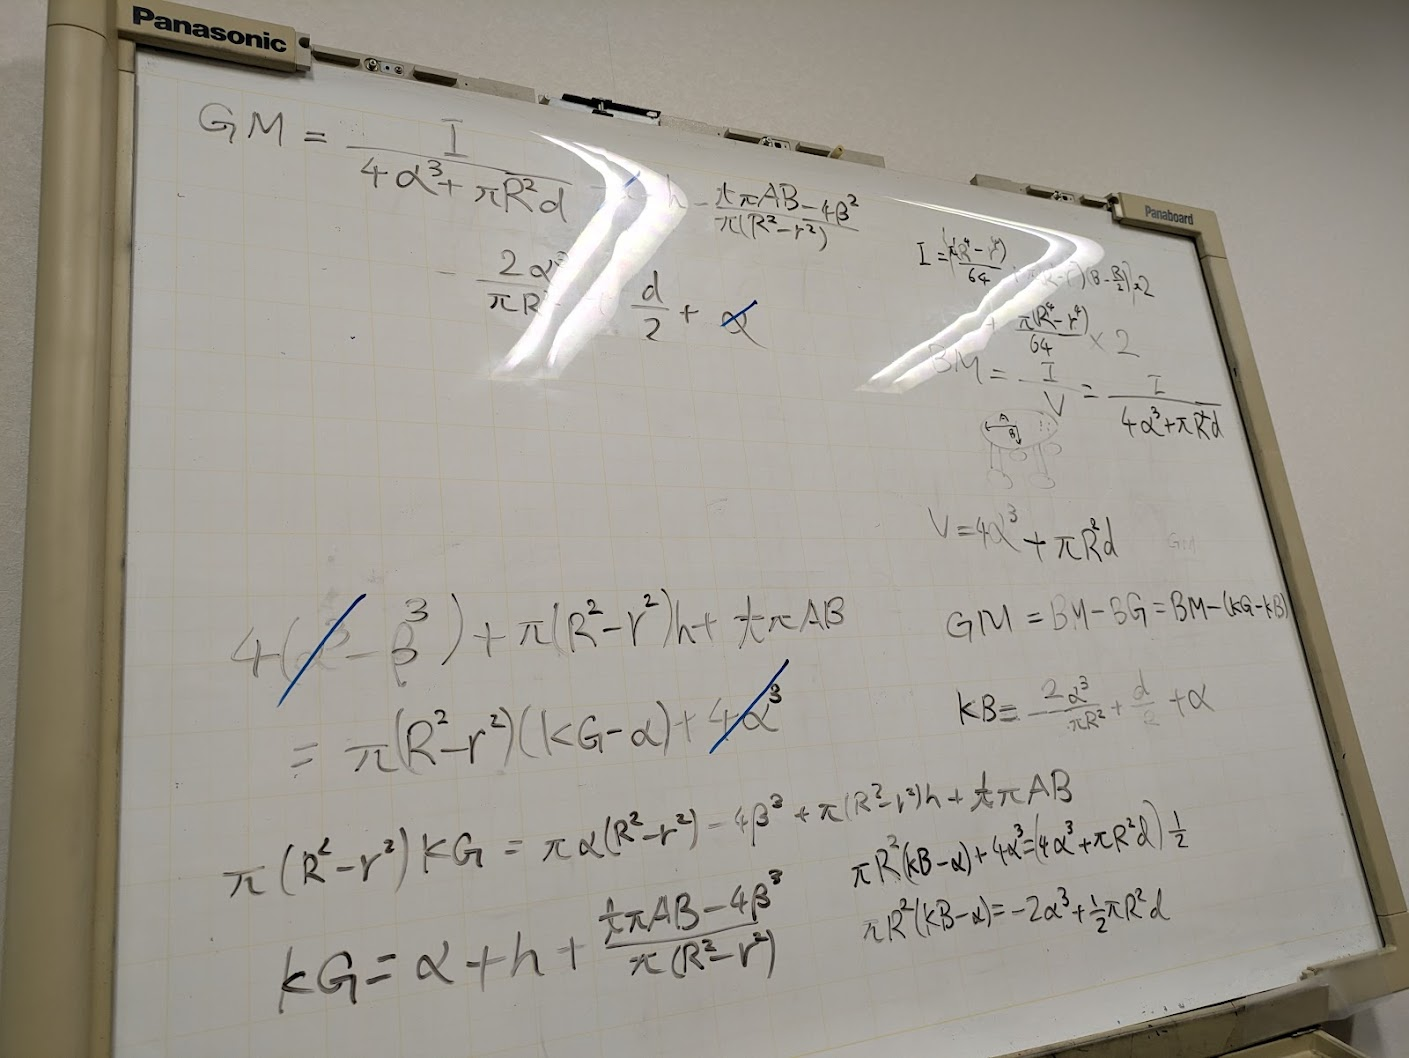
\includegraphics[width=0.7\linewidth]{gm_01.png}   
    \caption{GMの計算}
    \label{fig:gm_calculation}
\end{figure}

後で絶対使う計算式なので、\cref{fig:gm_calculation}を参考にして、GMの計算式を以下に示す。
\begin{equation}
    GM = KB + BM - KG
\end{equation}
\begin{equation}
    BM = \frac{I}{V}
\end{equation}
先に変数の定義を以下に示す。
\begin{itemize}
    \item $R$ : 円筒柱の外径
    \item $r$ : 円筒柱の内径
    \item $h$ : 円筒柱の高さ(バラストタンクまで含んだ長さであり、円筒部分は$h-\alpha$)
    \item $d$ : セミサブ浮体の喫水
    \item $A$ : 楕円の長辺半径
    \item $B$ : 楕円の短辺半径
    \item $M$ : 楕円形上部構造の重量+積載物の重量
    \item $\rho$ : 浮体を構成する材料の密度
    \item $\rho_w$ : 海水の密度
    \item $I$ : 断面2次モーメント
    \item $V$ : 水面下の体積
    \item $KB$ : 喫水面から底面までの距離
    \item $BM$ : 浮心から復元力の作用点までの距離
    \item $KG$ : 喫水面から重心までの距離
    \item $GM$ : メタセンター高さ
    \item $\alpha$ : バラストタンクの立方体外寸
    \item $\beta$ : バラストタンクの立方体内寸
\end{itemize}



\subsection{短辺方向のBMを出す}
今回設計するセミサブ浮体は円筒形なので、外径$R$, 内径$r$とすると断面2次モーメント$I$は以下の式で求められる。
\begin{equation}
    I_A = \frac{\pi (R^4-r^4)}{64}
\end{equation}
また、平行軸の定理より、楕円の短辺半径をBとしたときの断面2次モーメント$I_B$は以下の式で求められる。
\begin{equation}
    I_B = I_A + \frac{\pi}{4}(R^2 - r^2)(B-\frac{R}{2})^2
\end{equation}
以上より4本の円筒柱で構成されるセミサブ浮体の断面2次モーメント$I_{total}$は以下の式で求められる。
\begin{align}
    I_{total} &= 2 I_A + 2 I_B = \frac{\pi}{64}(R^4 - r^4)\times 2 + \left\{\frac{\pi}{64}(R^4 - r^4) + \frac{\pi}{4}(R^2 - r^2) (B-\frac{R}{2})^2 \right\}\times 2\\ 
    &= \frac{\pi}{16}(R^4 - r^4) + \frac{\pi}{2}(R^2 - r^2) (B-\frac{R}{2})^2
\end{align}
ちなみに、水面下の体積$V$は以下である。
\begin{equation}
    V = 4\alpha^3 + 4 \left( \frac{\pi R^2}{4} \right) (d-\alpha) = 4\alpha^3 + \pi R^2 (d-\alpha)
\end{equation}
よって、BMは以下の式で求められる。
\begin{equation}
    BM = \frac{I_{total}}{V} = \frac{\frac{\pi}{16}(R^4 - r^4) + \frac{\pi}{2}(R^2 - r^2) (B-\frac{R}{2})^2}{4\alpha^3 + \pi R^2 (d-\alpha)}
\end{equation}




\subsection{短辺方向のKBを出す}
セミサブ浮体の喫水をdとすると、以下の等式が成り立つ。
$$KB = \frac{水面下の体積モーメントの和}{排水容積}$$
つまり、
\begin{align}
    KB &= \frac{4\alpha^3\cdot \frac{\alpha}{2} + 4\frac{\pi R^2}{4}(d-\alpha)\cdot \frac{d+\alpha}{2}}{4\alpha^3 + \pi R^2(d-\alpha)}\\
    &= \frac{2\alpha^4 + \frac{\pi R^2}{2}(d^2 - \alpha^2)}{4\alpha^3 + \pi R^2(d-\alpha)}
\end{align}



\subsection{KGの導出}
重心Gは浮体全体の質量の中心である。底面を基準(高さ0)として、各パーツの質量モーメントの合計を総質量で割ることで$KG$を求める。
\begin{equation}
    KG = \frac{\sum (m_i \cdot z_i)}{\sum m_i} = \frac{m_{bal} \cdot z_{bal} + m_{col} \cdot z_{col} + M \cdot z_M}{m_{bal} + m_{col} + M}
\end{equation}
各項を代入すると、
\begin{equation}
    KG = \frac{\left( \rho \cdot 4(\alpha^3 - \beta^3) \right) \cdot \frac{\alpha}{2} + \left( \rho \pi(R^2-r^2)(h-\alpha) \right) \cdot \frac{h+\alpha}{2} + M \cdot z_M}{\rho \cdot 4(\alpha^3 - \beta^3) + \rho \pi(R^2-r^2)(h-\alpha) + M}
\end{equation}
分子を整理すると、$KG$は以下の式で表される。
\begin{equation}
    KG = \frac{2\rho\alpha(\alpha^3 - \beta^3) + \frac{\rho\pi}{2}(R^2-r^2)(h^2-\alpha^2) + M z_M}{4\rho(\alpha^3 - \beta^3) + \rho \pi(R^2-r^2)(h-\alpha) + M}
\end{equation}

\subsection{まとめ}
以上の結果より、GMは以下の式で求められる。
\begin{equation}
    GM = \frac{2\alpha^4 + \frac{\pi R^2}{2}(d^2 - \alpha^2)}{4\alpha^3 + \pi R^2(d-\alpha)} + \frac{\frac{\pi}{16}(R^4 - r^4) + \frac{\pi}{2}(R^2 - r^2) (B-\frac{R}{2})^2}{4\alpha^3 + \pi R^2 (d-\alpha)} - \frac{2\rho\alpha(\alpha^3 - \beta^3) + \frac{\rho\pi}{2}(R^2-r^2)(h^2-\alpha^2) + M z_M}{4\rho(\alpha^3 - \beta^3) + \rho \pi(R^2-r^2)(h-\alpha) + M}
\end{equation}


\end{document}